\section{引言}
\subsection{问题背景}

干燥是决定中药材成品品质的关键工序之一，热风烘干是应用最广的干燥方式。该方式通过调控烘房温湿环境，使热空气与药材表面进行对流换热与传质，从而将药材内部水分逐步蒸发去除。烘干过程通常包含\textbf{预热平衡}和\textbf{恒温干燥}两个阶段：预热阶段药材温度迅速升高、水分开始从表面逸出；恒温阶段烘房温度保持恒定，药材内部水分持续向外扩散。工艺参数选取不当容易导致干燥效率低、能耗高、成品品质不稳定等问题。

传统上，烘干工艺的确定依赖于大量正交试验，存在成本高、周期长的缺陷。随着数理分析与数值仿真方法的发展，通过建立药材内部传热传质的物理模型、以数值方法求解温度场与水分场，可以低成本、高效率地揭示干燥规律，为工艺参数优化提供依据。本题即以近似圆柱形的中药材为对象，要求建立数学模型回答四个递进的问题。

\subsection{问题重述}

\noindent 问题 1：某中药材近似为长 $25$ cm、半径 $2$ cm 的圆柱，烘干开始时药材温度为 $28$ °C、干基含水率为 $2.55$ kg/kg，烘房温度与空气水分浓度变化见附件 1。建立\textbf{预热平衡阶段}药材温度与水分浓度变化规律的数学模型（参数见附录 2），按表 1、表 2 格式给出 $100$ 至 $1800$ s 内、距药材中心 $0\sim2$ cm 处的结果，并将完整结果保存至 result1.xlsx。

\noindent 问题 2：烘干过程一般持续 2--3 天，预热平衡与恒温干燥阶段参数不同。建立\textbf{整个烘干过程}药材温度与水分浓度变化规律的数学模型（经验公式统一采用附录 3），按表 3、表 4 格式给出 3 h 内每隔 0.5 h、距中心 $0\sim2$ cm 处的结果，并保存完整结果至 result2.xlsx。

\noindent 问题 3：按烘干要求，药材各处水分浓度应低于 $0.15$ kg/kg，确定药材烘干所需时间（h）。按表 5 格式给出每隔 6 h、距中心每隔 0.5 cm 的水分浓度，并保存完整结果至 result3.xlsx。

\noindent 问题 4：实际烘干中药材因失水发生尺寸变化，根据附件 2（半径随时间变化）与附录 4 经验公式，确定药材的烘干时长。按表 6 格式给出水分浓度分布，并保存完整结果至 result4.xlsx。

本文的整体技术路线如图~\ref{fig:overall-technical-route} 所示。

\begin{figure}[htbp]
	\centering
	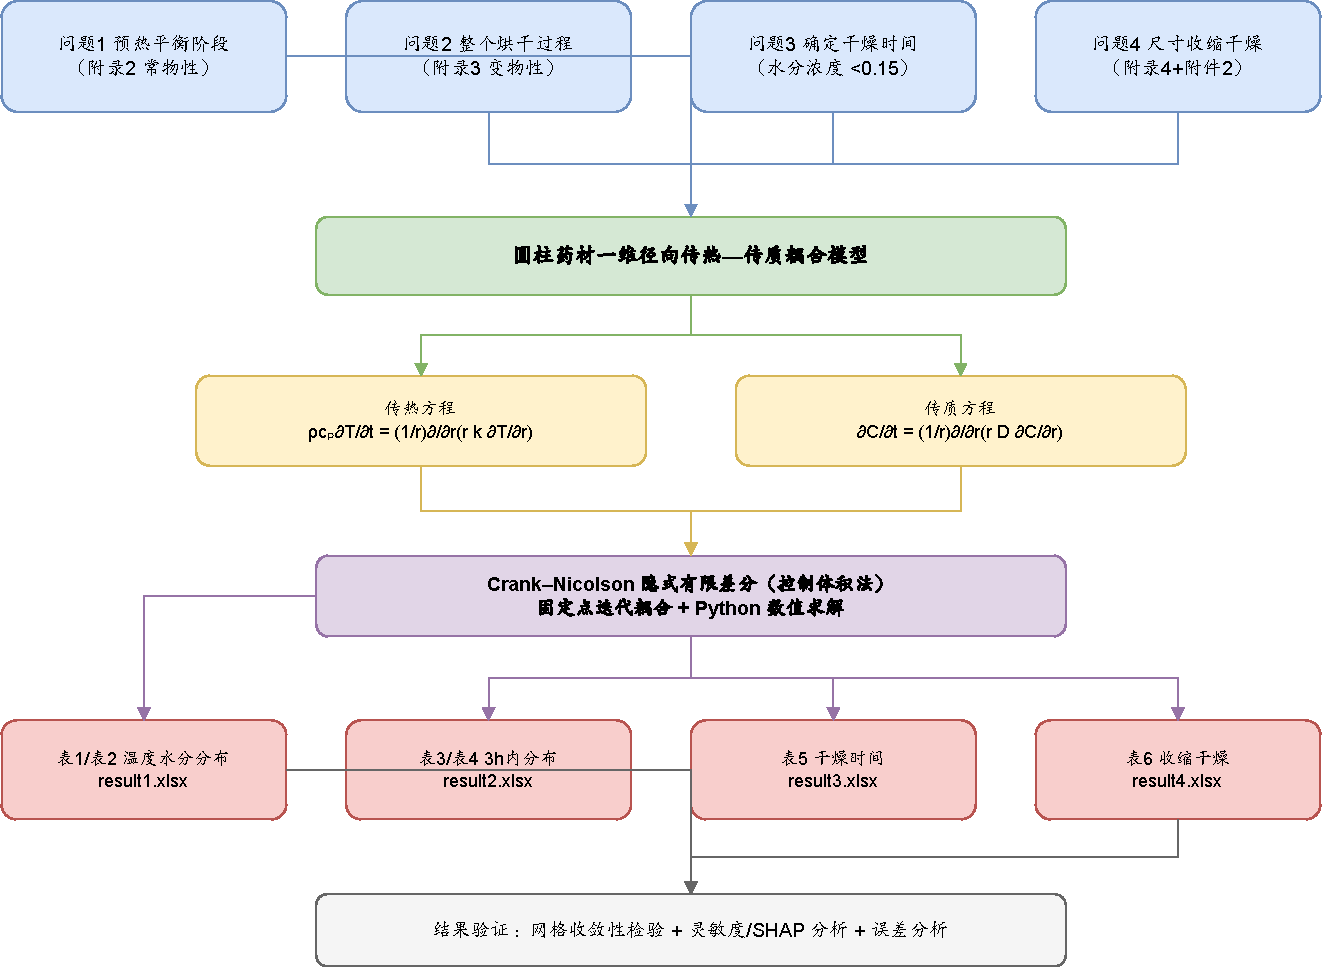
\includegraphics[width=0.96\textwidth]{texfile/figures/fig_route.pdf}
	\caption{整体技术路线图}
	\label{fig:overall-technical-route}
\end{figure}
